\chapter{Identifying Local Influencers and City-Level Communities}\label{chap3}

\setlength{\abovedisplayskip}{-10pt} \setlength{\abovedisplayshortskip}{-10pt}

\section{Background}
User's popularity on Twitter can be measured by how well the user is recognized by others, such as through others' mentions and follows. Understanding the location of popular users is needed for content recommendation and other use cases. For example, an advertising agency, that is performing a city-wide promotion, will be interested in users that serve important roles within that city such as the city's mayor. Generating crime statistics across cities could require focusing on local fire, police, and other emergency related influencers. Tracking sports could require tracking local football, basketball, baseball, and others relevant to the city of interest. 

The standard approach first geocodes a large number of users using each user's self-reported location. Second, the users whose locations map to within $x$ miles of the city of interest are used to establish the city-level community. As has already been noted in Chapter 2, the biggest obstacle to this approach is the lack of a good geocoding solution. 

In contrast, our approach does not require geocoding and instead leverages the power of Google search along with the follow structure on Twitter. We found that querying for (city, state, plus keyword `Twitter') is likely to return Twitter influencers that are specific to the city (geo-influencers). The geo-influencer's followers form the basis of a city-community. The benefit is that many of the followers may not contain a geocodable self-reported location, but make it in as part of our approach (this is because following a geo-influencer serves as a strong indicator of the follower's location). Following a local police department and local traffic updates serve as a strong indicator of the user's location even if the user does not list a geocodable self-reported location field. 
 
The Term Frequency-Inverse Document Frequency (TF-IDF), where the Term Frequency measures the number of follows by the community, is used to produce a ranked list of most popular geo-influencers. In this way, by fusing the power of Google for finding initial geo-influencers and the crowd-sourcing power of the underlying Twitter community, we can associate hundreds of additional city-level geo-influencers and use these to further refine the city-community. A ranking of national-level influencers are those with followers across multiple city-level communities.

\section{Related Research}

There is a great amount of research related to Twitter user's activity, popularity, and influence [\ref{appendix:2.1}]. Activity measures actions that a user takes (such as tweets, retweets, mentions, and replies); influence measures whether user's actions are capable of affecting other users' actions in the network; and popularity measures how well the user is recognized such as through others users' mentions and follows. In this research, we are focusing on popularity through other user's follows. This work is related to Location-Aware Influence Maximization (LAIM) [\ref{appendix:2.2}, \ref{appendix:2.3}], where the goal is to identify top k users to maximize the expected number of influenced users in a specific geographical area. 

%In popularity ranking an essential step is to establish a community of users over which it is computed. 
Multiple features can be used to establish a community of users with some features in common [\ref{appendix:2.4}]. For example,  (i) structure-based features where two users both follow the same influencer [\ref{appendix:2.5}-\ref{appendix:2.8}], (ii) activity-based features such as how frequently and during what times the user is active [\ref{appendix:2.9}-\ref{appendix:2.11}], (iii) content-based features such as the type of users, topics, URLs being mentioned [\ref{appendix:2.12}-\ref{appendix:2.14}], and (iv) communication-based features such as retweet, reply, and mention [\ref{appendix:2.15}, \ref{appendix:2.16}]. 

The second step is to associate users with a geographical area (usually at the city-level). The user's location may be geocoded from the self-reported profile location or aggregated from coordinates in the user's tweets [\ref{appendix:1.1}]. For a user without location information, the median of user's friends' location can be used [\ref{appendix:1.11}, \ref{appendix:2.19}].% These approaches suffer due to a high level of noise associated with geocoding locations. For example, tweets with precise GPS coordinate point are limited to 1\% of the overall Twitter stream and may not refer to a user's home location [\ref{appendix:1.12}]. The self-reported profile location may be available for over a third of users, but needs to be geocoded and is prone to ambiguous locations like `Planet Earth' [\ref{appendix:1.2}].

Finally, once the communities and the underlying geographical locations are known, the ranking of the users for each geographical area can be done using traditional graph metrics such as degree centrality [\ref{appendix:2.22}], custom measures that for example punish spammers [\ref{appendix:2.23}], and variations on PageRank [\ref{appendix:2.24}-\ref{appendix:2.26}]. 

A recent paper, that is most directly related to our research, explores the problem of identifying relevant geo-influencers across three US cities: Boston MA, Bristol CT and Seattle WA [\ref{appendix:2.26}]. Their network was built using social activity based interactions retweet, reply, and mention present in over five billion tweets. They relied on self-reported profile location information for extracting a ranked list of influential users whose location is within 100km of the city of interest. The ranking was performed via several modified PageRank based algorithms. They showed that self-reported locations were needed for filtering out global users that are not from the area such as @YouTube. However, it was also shown that limiting users within $x$ miles of the location of interest would filter out other important users, such as @Patriots, that had a strong local connection spanning beyond 100 km.

We propose a novel way of performing a targeted collection that results in a community of users for each city location. For each city, the communities stem from an initial pool of influential users identified via automatic Google searches. Our approach does not rely on any location information. In this way, each community may contain passive readers that do not tweet and users with no location information. Most importantly our city communities are made up of followers of geo-influencers that are known to be associated with the city of interest. A modified TF-IDF measure results in ranked lists that perform well against hand-labeled data including data from [\ref{appendix:2.26}], but the overall collection requirements are magnitudes smaller.

\section{Approach}
Given a city of interest and a list of other cities from which to distinguish, our approach will follow the process outlined in Fig. 3.1. The figure shows four main steps: (1) Google search to discover known geo-influencers for each city, (2) ordinary followers of geo-influencers from step 1 are used to establish a city community, (3) collect friends of the city community from step 2, and (4) a modified TF-IDF measure is used to identify geo-influencers from step 3. In our work, we define `an ordinary follower' as one who has between 20 and 100 friends, less than 500 followers, not verified by Twitter, without a URL, and that does not generate over five tweets per day since created. An influencer is simply a user with at least 500 followers.

Steps 1-3 shown on the left side of Fig. 3.1 are repeated for each city after which step 4, illustrated on the right, is applied. Each component of the process from Fig. 3.1 is described in more detail in the subsections below.

\begin{figure}[!t]
\centering
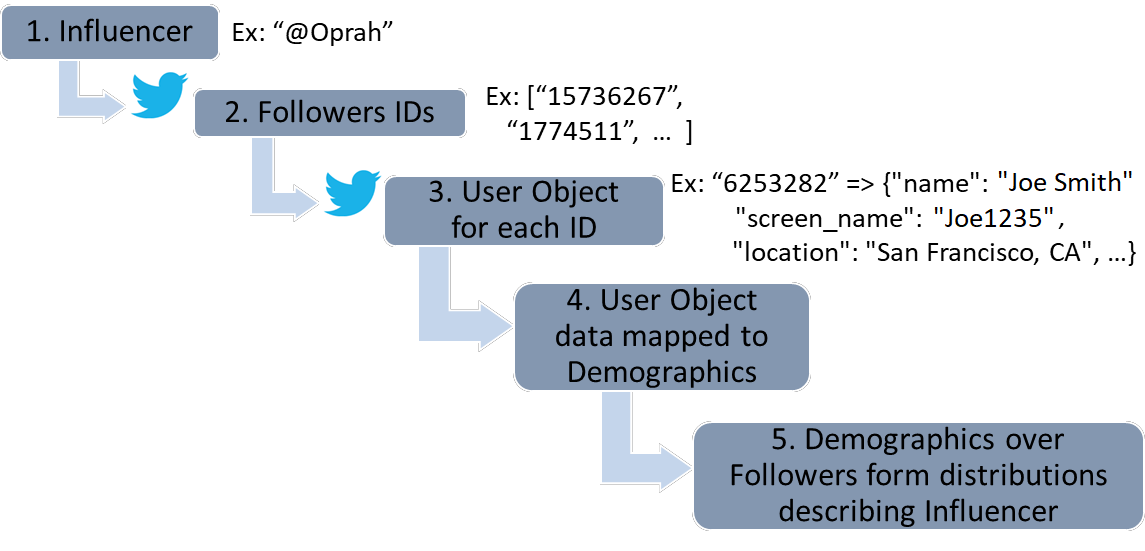
\includegraphics[width=4in]{Fig1}
\caption{Top N geo-influencers extracted from K Cities}
\label{fig_ch3_1}
\end{figure}

\noindent\textbf{Step 1: Google Queries for getting the Initial Geo-Influencers}-- Given a query that consists of (city, state, `Twitter') (and an optional keyword such as `Sports') Google returns a list of URLs. In the first 100 Google hits, our interest is in the following URL structure: `https://twitter.com/' + screenname + `?lang=en'. We record the screenname and the associated URL hit number. In this manner, Google search associates influencers with a city. In our work, the top ten influencers are used. By utilizing optional keywords, such as `News' or `Sports', we can focus on the geo-influencers by topic. For example, the query `Syracuse, NY Twitter News' results in the top three news-related influencers: @SyracuseUNews, @syracusedotcom, and @NewsChannel9. 

\noindent\textbf{Step 2: Initial Geo-Influencers to City Community}-- Twitter API is used to collect followers of initial geo-influencers; thus forming the basis of the city community. According to a 2016 Twitter SEC filing, approximately 8.5\% of all Twitter users are bots [\ref{appendix:2.27}]. Bots have many connections and post many messages. Thus, to avoid/minimize bots we focus on ordinary followers (one of the criteria is not posting over five messages a day). To focus on the users that are interested in a single city, we also ensure that city-communities are disjoint, i.e., no user belongs to two or more communities.  

\noindent\textbf{Step 3: City Community to Additional Geo-Influencers}-- Twitter API is used to collect friends of users that make up the city community; users with over 500 followers form a pool of additional `potential' geo-influencers; potential because influencers which are popular across multiple cities may be included (TF-IDF measure helps filter these out).

\noindent\textbf{Step 4: Ranking via TF-IDF}-- As mentioned earlier, traditional approaches find the influencers using network based methods, such as the degree centrality or PageRank. In our research, we apply TF-IDF, which is intended to reflect how important a word is to a document in a corpus. To apply TF-IDF measure it was critical to have well defined city communities (those consisting of users that are from the city). For each city, a document is made up of all potential geo-influencers that the city community has made a connection to. The process shown on the left in Fig. 3.1 builds such a document for each city.

Let C represent the set of all cities, community($c_v$) return the set of ordinary followers that make up the community for city $c_v$, and friends($o_w$) return the set of influencers that the user $o_w$ follows:

\begin{itemize}
\item C = \{$c_1$, $c_2$, ..., $c_k$\}
\item community($c_v$) = \{$o_1$, $o_2$, ..., $o_m$\}
\item friends($o_w$) = \{$u_1$, $u_2$, ..., $u_n$\}
\end{itemize}

Term frequency for user $u_x$ and community $c_v$ corresponds to total friend connections to user $u_x$ within community divided by total friend connections: 

\begin{equation}
TF(u_x, c_v) = \frac{\sum_{o \epsilon community(c_v)} |u_x \epsilon friends(o)|}{\sum_{o \epsilon community(c_v)} |friends(o)|}
\end{equation}

As an example, given community($c_1$) = \{$o_1$, $o_2$, $o_3$\} where friends($o_1$) = \{$u_1$, $u_2$\}, friends($o_2$) =\{$u_2$, $u_3$\}, and friends($o_3$) = \{$u_1$, $u_2$, $u_3$\}: TF($u_1$, $c_1$) =(1+0+1)/(2+2+3) = 2/7, similarly TF($u_2$, $c_1$) = 3/7 and TF($u_3$, $c_1$) = 2/7.

Inverse document frequency is given by the total number of cities divided by the number of cities user $u_x$ has a connection to (cities where that user is mentioned more than once):

\begin{IEEEeqnarray}{rCl}
IDF(u_x) & = & \log \biggl(\frac{|C|}{\sum_{c_v \epsilon C}|\{TF(u_x, c_v) > 0\}|} \biggr)
\end{IEEEeqnarray}

As an example, given another community($c_2$) = \{$o_4$\} where friends($o_4$) = \{$u_1$, $u_4$\}: IDF($u_1$) = log(2/(1+1)) = 0 and IDF($u_4$) = log(2/(0+1)) = log(2).

Combining formula 1 and 2 gives a formula for ranking a potential influencer $u_x$ for community $c_v$:

\begin{equation}
TF-IDF(u_x, c_v) = TF(u_x, c_v)*IDF(u_x)
\end{equation}

\section{Data}
Using the data from the 2016 Census Bureau we focused on known cities in the USA. We built a set of cities by initially starting with the most populous city and incrementally adding other most populous cities as long as they were at least 30 miles apart from cities already in the set. This ensured that the selected cities were geographically spread apart. The set so obtained contained 264 (city, state) pairs.

The process in Fig. 3.1 was used to generate three datasets based on three different keywords that made up the Google query: (i) Twitter, (ii) Twitter News, and (iii) Twitter Sports. Out of 264 cities, only 64 cities contained at least ten geo-influencers for each search type. Followers of geo-influencers were used to establish each city community. The followers that simultaneously follow many geo-influencers were prioritized. It was required that each city community have at least 100 and at most 1000 users. Fig. 3.2 shows the collection process for the network associated with each city and the corresponding maximum network size.

\begin{figure}[!t]
\centering
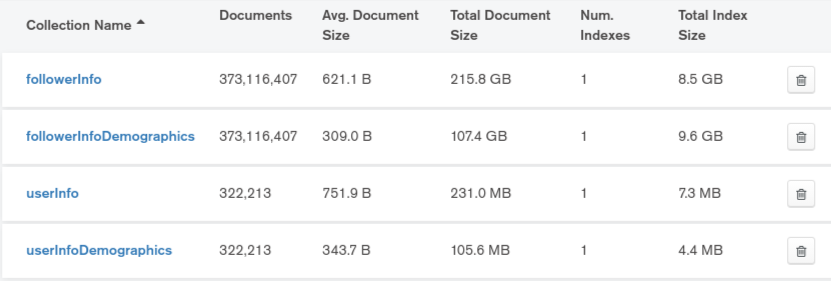
\includegraphics[width=4in]{Fig2}
\caption[Collection from seed, to city-community, to set of influencers]{Collection process from initial influencers to city-level community to a new set of influencers (drawn to scale)}
\label{fig_ch3_2}
\end{figure}

In addition to the three datasets described above, we obtained the fourth dataset where the city community is made up of users whose self-reported locations were verified via geocoder (using Google Maps API\footnote{https://developers.google.com/maps/documentation/geocoding}) to within 10 miles of city's (latitude, longitude). For this dataset, ordinary followers were selected from the followers of major news outlets: ABC, Politico, PBS, WSJ, Fox News, Reuters, CNN, and MSNBC. For each city community, we collected at least 100 users but at most 1/500 of the city's population. Out of the 64 cities covered by the other three datasets, only 19 cities provided a large enough sample size. These 19 city communities across the four datasets were: Charlotte NC, Washington DC, Wichita KS, Tucson AZ, Denver CO, Madison WI, San Diego CA, Syracuse NY, Lansing MI, Toledo OH, Boston MA, Columbia MO, Chicago IL, Springfield MO, Rochester NY, Lubbock TX, Atlanta GA, Topeka KS, and Albany NY.

Comparing results from the first three datasets showed the effect of differing queries, i.e., how the resulting communities differ in geo-influencer ranking. The fourth dataset allows us to compare how the city community generated via geo information differs from community based on follow connections to Google identified influencers. Table 3.1 summarizes the four datasets collected across these 19 cities. Table 3.1 shows the number of users, average, and standard deviation per community. From the table, we see that Dataset 4 has a high standard deviation, i.e., due to bigger samples for bigger cities. Dataset 3, related to `Twitter Sports', has a smaller community than the more general topics: `Twitter' and `Twitter News'.

\begin{table}
\small
\renewcommand{\arraystretch}{1.2}
\caption[Dataset Statistics across 19 Cities that occur within each dataset.]{Dataset Statistics across 19 Cities that occur within each dataset. The total number of users across the 19 city-communities is shown as well as the average number of users per city-community and the associated standard deviation.}
\label{table_ch3_1}
\centering
\begin{tabular}{|c|c|c|c|c|}
\hline
\bfseries Set & \bfseries Seed Type & \bfseries Avg & \bfseries Stnd & \bfseries Total \\
\hline
D1&Google using Twitter&692.21&203.52&13152\\
\hline
D2&Google using Twitter News&728.95&198.35&13850\\
\hline
D3&Google using Twitter Sports&516.32&324.30&9810\\
\hline
D4&Major National News&726.79&944.03&13809\\
\hline
\end{tabular}
\end{table}

\section{Evaluation}

\subsection{Impact of Keyword in Google query on Final Rank}

\begin{figure}[!t]
\centering
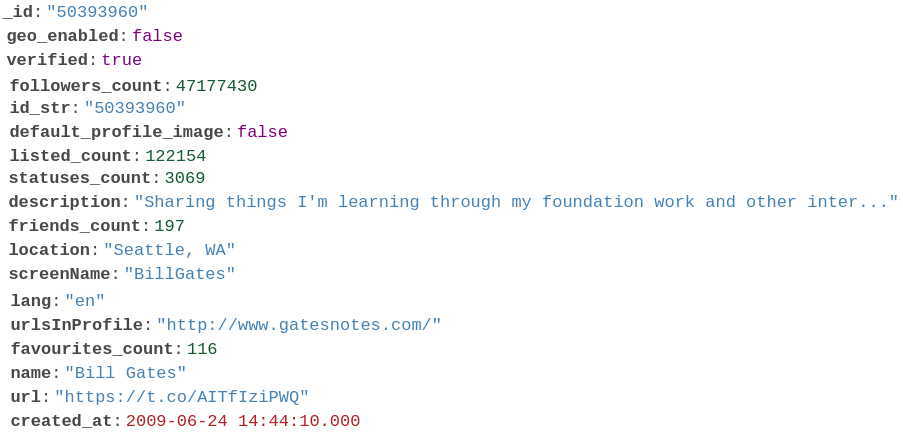
\includegraphics[width=5in]{Fig3}
\caption[Seed vs. Top Ranked Influencer Overlap Venn Diagram across 64 cities]{Seed Twitter User Overlap (left) vs. Top Ranked User Overlap (right) across 64 cities for the three search types). While the initial queries produce an initial set of influencers (seed) that differ (shown on the left), the resulting influencers that are extracted from city-level communities formed from seed have quite a bit of overlap (shown on the right). This illustrates that the method is robust in that different influencers can be used as a seed to get to the same end result (as long as the initial influencers are indeed local to the city of interest).}
\label{fig_ch3_3}
\end{figure}

We analyzed the first three datasets. The ground truth, in this case, are the geo-influencers using Google search. Each dataset contained 640 geo-influencers across 64 cities (1920 for all three datasets). Venn diagram in Fig. 3.3 (left) shows 79 out of 1920 or 4.1\% of geo-influencers associated by Google overlap across three search types with more overlap between Twitter and Twitter News. Ranked list via TF-IDF, Venn diagram of Fig. 3.3 (right) shows a more significant overlap, 297 out of 1914 or 15.5\% of users. The figure shows that on average more than half of ranked geo-influencers overlap (with Twitter and Twitter News being most aligned). This illustrates that different initial geo-influencers can lead to similar final rankings.

\subsection{Performance against Google Ranked Geo-Influencers}

Google is driven by those webpages that a user is most likely to click on while the number of followers drives Twitter's popularity. In the majority of cases we have found that there is an overlap between Google associated users and top-ranked users via TF-IDF, especially as $n$ increases. We calculated the ratio of overlap between the two as:

\begin{equation}
Overlap(X(c_v), Y(c_v,d,n)) = \frac{|X(c_v) \cap Y(c_v,d,n)|}{|X(c_v)|}
\end{equation}

Where X($c_v$) refers to a set of known geo-influencers that are associated with city $c_v$ from Google and Y($c_v$, $d$, $n$) refers to top $n$ ranked influencers stemming from the TF-IDF measure for city $c_v$ and dataset $d$. 

The top ten geo-influencers across three Google search types are combined providing a larger set to compare against (24.58 geo-influencers on average). Fig. 3.4 shows, for each dataset, the average percent of Google geo-influencers confirmed by each query type as the ranked list grows in size. The metric is averaged across 19 cities that are present in each of the four datasets. Despite each dataset representing slightly differing communities, due to having been formed using different seeds, we see that they all confirm a similarly large portion of geo-influencers that were deemed relevant by Google with generic Twitter search type working the best.

\begin{figure}[!t]
\centering
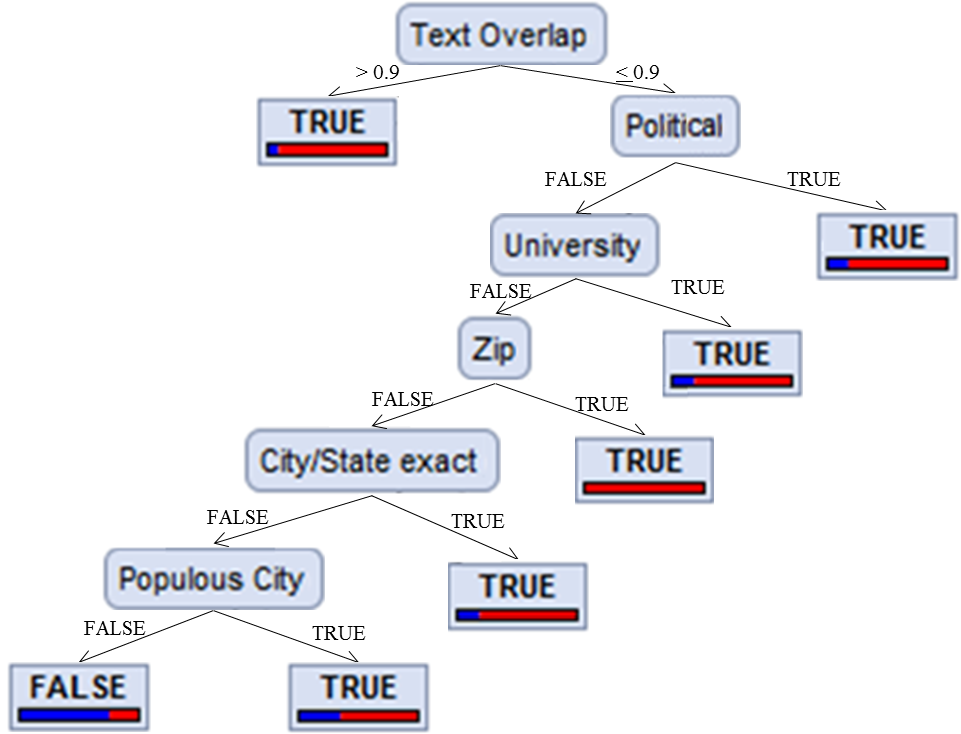
\includegraphics[width=4in]{Fig4}
\caption[Percent of Google geo-influencers confirmed by each query type]{Percent of Google geo-influencers confirmed by each query type as the ranked list grows in size. Followers of major news that were verified via geocoder follow similar influencers as returned from Google.}
\label{fig_ch3_4}
\end{figure}

In a similar fashion, Table 3.2 shows the top 30 geo-influencers using TF-IDF vs. top ten geo-influencers for each Google search type. The last row is a combination of the top ten Google geo-influencers across datasets D1-D3, also used in Fig. 3.4. Ratios in bold highlight the best aligning datasets. It could be argued that each dataset simply confirms the same initial seed that was used to establish the dataset. D4 was established, to illustrate that communities established without leveraging Google would also confirm them. Communities from D4 were established from self-reported locations of followers following major news influencers and hence did not utilize Google in any way. Despite this D4 had a high overlap for Twitter News search type (0.61, this overlap helps confirm that the proposed approach can work in a similar fashion as the one that relies on geocoding).

\begin{table}
\small
\renewcommand{\arraystretch}{1.2}
\caption{Overlap for Geo-Influencers from Google vs. Dataset}
\label{table_ch3_2}
\centering
\begin{tabular}{|c|c|c|c|c|}
\hline
\bfseries Search Type (X) & \bfseries D1 & \bfseries D2 News & \bfseries D3 Sports & \bfseries D4 News \\
\hline
Twitter&\bfseries 0.69&0.62&0.37&0.55\\
\hline
Twitter News&0.71&\bfseries 0.74&0.47&0.61\\
\hline
Twitter Sports&0.12&0.12&\bfseries 0.28&0.08\\
\hline
all&\bfseries 0.43&0.42&0.33&0.34\\
\hline
\end{tabular}
\end{table}

Next, we focus on Google geo-influencers that do not make it into ranked lists even for very large n. For instance, for n=1000 there were 67 such geo-influencers. We checked each of the 67 geo-influencers by hand. 37 out of 67 geo-influencers were found accurate, but all had fewer than 500 followers to be considered by our method. These referred to local high schools, local businesses, small local sports teams related to tennis, volleyball, and others. To incorporate these geo-influencers, we would need to change our threshold for influencer from 500 to 100 followers.

Next, examples of Google geo-influencers that were found inaccurate. @CityofToledo has never tweeted, with 105 followers, being in the fourth search result for the query `Toledo OH Twitter' (this is probably due to close overlap in keywords with @city\_of\_toledo the first search result and official city account). Some influencers have a national follower base, but are associated with a single city such as @RiddellSports associated with `Chicago, IL Twitter Sports'. Google search results fluctuate over time with about two-thirds of the 67 accounts no longer recommended after the search was repeated about a month later. Hence verification is still recommended for optimal results when establishing initial geo-influencers from which each city community is to be established.

\subsection{Communities via Location vs. Google Seed}

Dataset D4 was established using followers of major national news outlets whose self-reported location could be associated with the city of interest. The issue with self-reported locations is that less than a quarter of all users had locations that could be geocoded. Also, we found geocoding errors for example `Salem' was associated with `Salem, MA', but often the location referred to Salem which is in India. As a result, we focused on high confidence locations that specify both city and state, but such locations were challenging to find for smaller cities despite collecting on millions of users.
 
The benefit of datasets D1-D3 is that they were assembled much quicker than D4 and they covered many more cities with more users per city. For users in D1-D3, over 64 city communities, the percent of users with the non-empty self-reported location was only 28.2\%. For those users that did specify their location, on average 41.6\% contained the city name associated by our method, thus illustrating that these communities are well structured.

\subsection{City Level Evaluation}
\begin{table}
\small
\renewcommand{\arraystretch}{1.2}
\caption{Top 30 Geo-Influencers extracted from each Dataset}
\label{table_ch3_3}
\centering
\tabcolsep=0.09cm
\begin{tabular}{|c|c|c|c|}
\hline
\bfseries D1&\bfseries D2 News&\bfseries D3 Sports&\bfseries D4 News\\
\hline
\bfseries marty\_walsh&boston25&\bfseries cityofboston&visitbostoncity\\
\hline
\bfseries cityofboston&\bfseries 7news&hiddenboston&\bfseries cityofboston\\
\hline
\bfseries bostondotcom&\bfseries wcvb&\bfseries wcvb&\bfseries bostondotcom\\
\hline
bostontweet&\bfseries bostondotcom&\bfseries marty\_walsh&\bfseries marty\_walsh\\
\hline
mbta&\bfseries bostonpolice&eatboston&bostontweet\\
\hline
onlyinbos&onlyinbos&\bfseries bostondotcom&mbta\\
\hline
\bfseries 7news&massstatepolice&bostontweet&bostonmagazine\\
\hline
\bfseries bostonpolice&bostonglobe&mbta&\bfseries bostonfire\\
\hline
bostonmagazine&mbta&bostonmagazine&\bfseries 7news\\
\hline
massgovernor&\bfseries cityofboston&boston25&\bfseries bostonpolice\\
\hline
\bfseries wcvb&\bfseries marty\_walsh&massstatepolice&mayortommenino\\
\hline
hiddenboston&massgovernor&massdot&massdot\\
\hline
boston25&bostonmagazine&\bfseries 7news&eatboston\\
\hline
bostonglobe&bostontweet&\bfseries bostonfire&bplboston\\
\hline
massstatepolice&\bfseries wbz&massgov&\bfseries wcvb\\
\hline
bostinno&985thesportshub&theimproper&bostonglobe\\
\hline
bostonpwd&\bfseries nhlbruins&\bfseries bostonpolice&massgovernor\\
\hline
\bfseries nhlbruins&scottzolak&bosbizjournal&massgov\\
\hline
stoolpresidente&jerry\_remy&\bfseries wbz&boston25\\
\hline
edelman11&stoolpresidente&mbta\_alerts&massstatepolice\\
\hline
\bfseries wbz&wilfork75&massema&bostonparksdept\\
\hline
theimproper&hiddenboston&mbtatransitpd&bostinno\\
\hline
\bfseries bostonfire&justamasshole&eaterboston&theimproper\\
\hline
\bfseries redsox&lowellsunnews&massgovernor&hiddenboston\\
\hline
\bfseries celtics&\bfseries celtics&harveywcvb&\bfseries wbz\\
\hline
bos311&edelman11&universalhub&visitma\\
\hline
universalhub&bostinno&mayortommenino&universalhub\\
\hline
bostonbtd&theimproper&bostinno&onlyinbos\\
\hline
jerry\_remy&toucherandrich&985thesportshub&bostoncalendar\\
\hline
\bfseries bostonherald&nesn&fredtoucher&bostonschools\\
\hline
\end{tabular}
\end{table}

Evaluation in [\ref{appendix:2.26}] listed ground truth for Boston MA via these 20 geo-influencers: (i) News = wcvb, bostondotcom, cbsboston, 7news, bostonherald, (ii) Sports = redsox, celtics, nhlbruins, thebostonpride, bostoncannons, (iii) Gov = marty\_walsh, cityofboston, bostonpolice, bostonfire, masddot, and (iv) University = bu\_tweets, harvard, mit, berkleecollege, northeastern (influencer cbsboston renamed to wbz). The top five for the best performing ranked list from [\ref{appendix:2.26}] contained: Patriots, BostonGlobe, OnlyInBOS, RedSox, and NHLBruins (so in their approach the last two matched the ground truth). For our approach, table 3.3 shows the top 30 geo-influencers (those in bold match the ground truth).

Our approach carries as many as four matches in the top five and as many as twelve matches in the top thirty geo-influencers. This compares favorably to the results reported in [\ref{appendix:2.26}]: two matches in the top five and eleven matches in the top thirty influencers. None of our ranked lists incorporate high-level influencers such as @YouTube. Furthermore, our approach allows targeted city collection which results in an overall network being orders of magnitude smaller. As was shown in Fig. 3.2 there are at most 100,000 users collected per city. 

A number of geo-influencers overlap across the four datasets. This again reinforces that similar results can be achieved via differing city communities as long as those communities are local to the city. What differentiates communities is that the ranking will be slightly tilted towards the query. For example, Table 3.4 shows geo-influencers, and the position in the ranked list of 1000, that contain the keyword `Celtics' (a popular basketball team associated with Boston). As expected, D3 produces the most sports related influencers (because query also contained `sports').

\begin{table}
\small
\renewcommand{\arraystretch}{1.2}
\caption{From each Dataset Top Geo-Influencers containing keyword Celtics}
\label{table_ch4_4}
\centering
\tabcolsep=0.13cm
\begin{tabular}{|c|c|c|c|}
\hline
\bfseries D1&\bfseries D2 News&\bfseries D3 Sports&\bfseries D4 News\\
\hline
celtics: 25&celtics: 25&bdcceltics: 149&celticsblog: 304\\
\hline
celticslife: 525&celticslife: 115&nbcsceltics: 199&nbcsceltics: 386\\
\hline
&&celtics: 226&celticslife: 424\\
\hline
&&r\_bostonceltics: 261&bdcceltics: 483\\
\hline
&&celticsviews: 293&celtics: 975\\
\hline
&&celticsfanclub: 596&\\
\hline
\end{tabular}
\end{table}

\section{Geo-Influencer Collection Runtime}

Typically it is assumed that the social graph has already been collected and then different algorithms use its structure and various features in an attempt to identify the most important nodes. The algorithms are evaluated based on accuracy and runtime. We noticed that the algorithm runtime is negligible compared to the data collection time i.e. it is not uncommon for a researcher to have spent a year collecting the dataset, a dataset that cannot be fully shared with others (only unique ids can be shared and crawling on ids can take about as long as starting a new collection from scratch), and the dataset may not work all that well for a scenario that targets a certain demographic.

Up to 1\% of all Twitter message traffic can be collected using the unfiltered stream of tweets (from our experiments around 4 million tweets a day). This may seem like a lot of data, but for a specific use-case such as the 2014 annexation of Crimea by Russia, there might not be that many messages from the area of interest. The method proposed in this chapter is useful for identifying influencers and corresponding user communities from a particular geographic area. As an illustration, we show the expected collection times for three methods:
\begin{itemize}
\item  M1: using the union of followers from multiple geo-influencers
\item M2: using followers of a well-known influencer (national or global like)
\item M3: using message traffic
\end{itemize}

For influencers, the self-reported locations of the followers are analyzed. For message traffic, the self-reported locations of the users that generated the message are analyzed. For this illustration, we are interested in forming communities for cities: Syracuse and Buffalo of USA. The users whose self-reported location matches one of the cities are recorded. Each self-report location is turned to lowercase and it is checked whether the city name is present within it.

The geo-influencers associated with a city are found via automated Google search. All of the Twitter influencers identified in the top 100 URLs by Google are utilized. %Here are the geo-influencers associated with:

\iffalse
\begin{itemize}
\item Buffalo (28 total): DAErieCountyNY, NWSBUFFALO, BfloBizFirst, SPECNewsBuffalo, WBFO, BPDAlerts, RedandBlack716, BFLO\_CC, Buffalo\_Schools, SURJBuffalo, markpoloncarz, USACE\_Buffalo, BuffaloSewer, BuffaloBills, MobBuffalo, BuffaloSabres, wnymedia, IIBuff, news4buffalo, BuffaloNiagara, ECDOH, WGRZ, TheBuffaloNews, MayorByronBrown, buffalo\_ny, BuffaloEats, FBNY\_WNY, WKBW
\item Syracuse (28 total): VisitSyracuse, SPECNewsCNY, Cusememes, LO\_Syracuse, SyracuseAirport, dailyorange, CNYCentral, syrbasketball, SyracusePolice, NYSFair, CuseWBB, chrsbakr, AndrewDonovan, SyracuseOn247, Cuse\_Tennis, SyracuseU, Stephen\_Bailey1, Cuse\_MBB, NewsChannel9, BenWalsh44, OnondagaCounty, Cuse, CuseFootball, AdrienneSmithTV, SyracuseUNews, syracusedotcom, syracuseITC, Syracuse1848
\end{itemize}
\fi

All of the followers for these geo-influencers were collected for each city; for Buffalo\footnote{Followers collected over Buffalo geo-influencers (28 total): DAErieCountyNY, NWSBUFFALO, BfloBizFirst, SPECNewsBuffalo, WBFO, BPDAlerts, RedandBlack716, BFLO\_CC, Buffalo\_Schools, SURJBuffalo, markpoloncarz, USACE\_Buffalo, BuffaloSewer, BuffaloBills, MobBuffalo, BuffaloSabres, wnymedia, IIBuff, news4buffalo, BuffaloNiagara, ECDOH, WGRZ, TheBuffaloNews, MayorByronBrown, buffalo\_ny, BuffaloEats, FBNY\_WNY, WKBW}, a total of 2767322 were processed vs. 1165345 for Syracuse\footnote{Followers collected over Syracuse geo-influencers (28 total): VisitSyracuse, SPECNewsCNY, Cusememes, LO\_Syracuse, SyracuseAirport, dailyorange, CNYCentral, syrbasketball, SyracusePolice, NYSFair, CuseWBB, chrsbakr, AndrewDonovan, SyracuseOn247, Cuse\_Tennis, SyracuseU, Stephen\_Bailey1, Cuse\_MBB, NewsChannel9, BenWalsh44, OnondagaCounty, Cuse, CuseFootball, AdrienneSmithTV, SyracuseUNews, syracusedotcom, syracuseITC, Syracuse1848} (some followers repeat across geo-influencers, number of unique followers were 1774172 vs. 566815, respectively). The collection time was 29.3 hours for Buffalo and 13.16 hours for Syracuse. Fig. \ref{fig_collectionRun} shows the number of unique followers that contain the city name in their self-reported location per 25000 followers for the two communities. The number of new followers with Syracuse in their self-reported location plateaus at around 20K. While the followers that contain Buffalo in their self-reported location continue to rise to 55K.

\begin{figure}[!t]
\centering
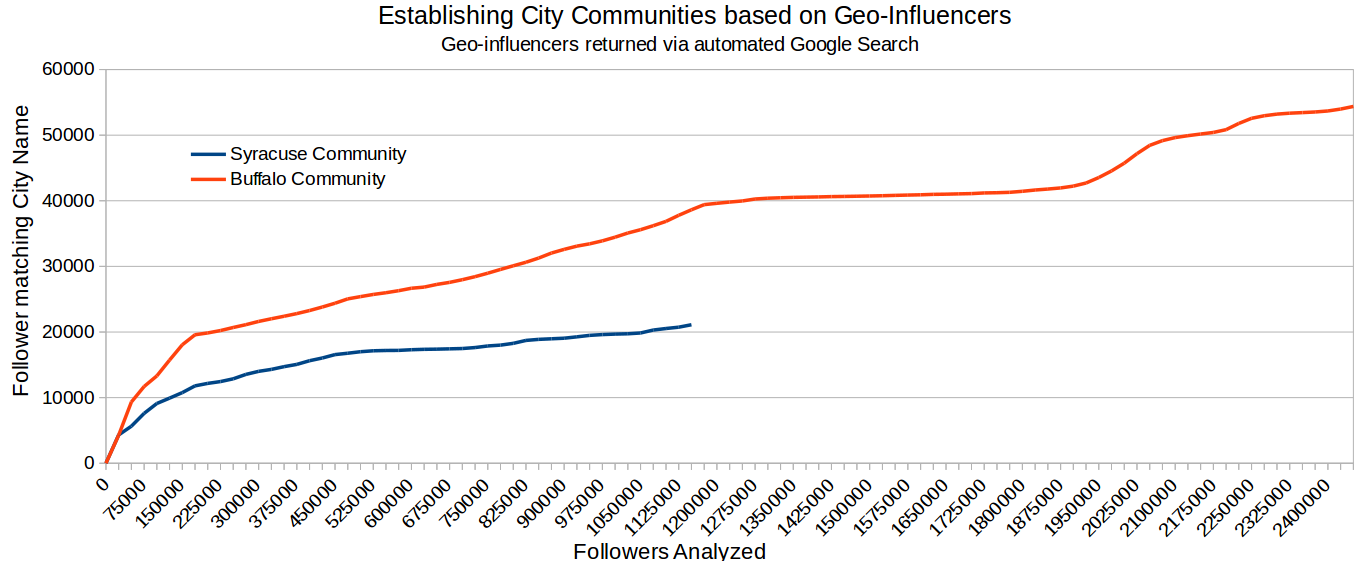
\includegraphics[width=5.6in]{Paper3Figures/FigCollectionRuntime.png}
\caption[Geo-Influencer Collection Runtime]{There is a large ratio of followers extracted with self-reported location matching the city of interest. Theoretically to process 25K in followers should take approximately 10 minutes. In this way in a relatively short time, in under 24 hours, a community of users that is representative of the city can be extracted. There is higher confidence in these users because they are known to follow a geo-influencer associated with the city as well as having the city in their self-reported location.}
\label{fig_collectionRun}
\end{figure}

Using influencer's followers it takes around 110 seconds to process 5000 followers\footnote{https://developer.twitter.com/en/docs/twitter-api/v1/rate-limits:\\GET followers/ids returns 5000 follower ids per minute, GET users/lookup can be used to process 900*100 ids per 15-minute interval or 100 followers per second. 60 seconds to collect 5000 followers ids plus 50 seconds to process ids gives 110 seconds.}. So theoretically, 3.92 million followers can be collected and processed daily. There are other factors impacting collection such as how quickly one can perform preprocessing and writes to a database which is why our collection times are a little different.

For method M2, using global/national like influencer, @NPR is used with 7.054M followers collected. This influencer was chosen because it is popular in the USA (a more global influencer like @CNN will perform worse as it will capture a smaller percentage of users for the cities in the USA). For message traffic a total of 10 million messages were collected (around 4 million messages daily). Table 3.5 shows how many users were extracted using each method divided by the total amount of time needed to perform the collection (time in hours). There is a much higher ratio of users for the city of interest from a collection that is focused on geo-influencers using method M1.

\begin{table}
\small
\renewcommand{\arraystretch}{1.2}
\caption{Average Number of Users (per hour) Matching City of Interest}
\label{table_abbr}
\centering
\begin{tabular}{|c|c|c|}
\hline
\bfseries users using method/collection time & \bfseries Syracuse & \bfseries Buffalo\\
\hline
method M1 based on geo-influencers & 21240/13.16=1614 & 56774/29.3=1938\\
\hline
method M2 based on global influencer & 1872/64.3=29 & 3994/64.3=62\\
\hline
method M3 based on message traffic & 283/57.36=5	 & 1048/57.36=18\\
\hline
\end{tabular}
\end{table}

Method M1 results in 21240 users for Syracuse and 56774 users for Buffalo. In comparison using message traffic to generate the same communities would require 21240/5/24=177 days and 56774/18/24=131 days respectively. For Syracuse, method M1 is 1614/5 = 322x and 1614/29 = 56x faster than method M2 and M3. For Buffalo, method M1 is 1938/18 = 107x and 1938/62 = 31x faster than method M2 and M3.

In a separate large collection of users based on followers of verified influencers (tracked by Twitter’s @verified) we collected 373 million profiles. This collection took over a year to complete. Across 373 million users, 42448 and 92276 contained Syracuse and Buffalo in their self-reported locations, respectively. This shows that the proposed M1 method can quickly identify roughly half of all Twitter users. The additional benefit in method M1 is that there is higher confidence in these users because they are known to follow a geo-influencer associated with the city as well as having the city in their self-reported location. 

Having identified the users that are representative of the demographic area, up to 3200 messages per user can be collected in a relatively quick amount of time\footnote{GET statuses/user\_timeline allows 900 requests per minute with each request providing up to 3200 Tweets (there is an additional limit to at most 100,000 requests per 24 hours)}. This will provide a larger set of relevant data than using the alternative methods we discussed. For example for Syracuse the 21240 users can be used to collect 15,206,890 messages and for Buffalo the 56774 users can be used to collect 54,913,648 messages. This is much more messages than can be collected in a day using the method M3 and these messages will be relevant to the geographic area of interest. The message creation times can be used to filter to the period of the incident that is wished to be analyzed. The messages can then be used with Natural Language Processing (NLP) to characterize and summarize the situation.

\section{Conclusions}

We have presented a novel method that utilizes geo-influencers for establishing city-level communities and then to identify additional geo-influencers, in a process that can repeat several times. Geo-influencers are at the city-level such as related to the city's mayor, local news, local police, and others. The initial set of geo-influencers is established via automatic Google queries. The followers of these influencers make up the resulting city-level communities; they have an interest in the city and for this reason, continue to follow updates related to the city posted by these geo-influencers. Our method does not require a geocoder to identify users that are local to a city.

We have confirmed that the majority of geo-influencers that Google finds relevant are confirmed via city-level communities built using a geocoder as well as through manual inspection. Communities, made up of users that reside in the city, allowed us to rank  thousands of influencers based on how influential they are in a given city. By targeting specific cities our approach can outperform comparable approaches while having an overall network and collection requirements that are orders of magnitude smaller. 